% Bibliography
\clearpage
\phantomsection\
\addcontentsline{toc}{section}{References}
\markboth{References}{References}
\section*{References}
\printbibliography[heading=none]

% --- Appendix ---
\clearpage
\appendix
\refstepcounter{section}
\setcounter{subsection}{0}
\phantomsection~\addcontentsline{toc}{section}{Appendix}
\markboth{Appendix}{Appendix}
\begin{center}\huge\bfseries Appendix\end{center}

\refstepcounter{subsection}
\subsection*{Requirements List}\label{app:req-list}
\subsubcetion{Organized by Requirement Type} \\ \\
\begin{footnotesize}
  \textsc{functional requirements}
    \begin{itemize}
        \item \textsc{FR-01 process orchestration engine} --- The system shall execute workflow models by dispatching tasks to human or software actors according to model control flow and business rules.
        \item \textsc{FR-02 parameterized subprocesses} --- The system shall support parameterized subprocesses and rules so behavioral variants can be expressed without altering the underlying process structure.
        \item \textsc{FR-03 human-machine task orchestration} --- The system shall coordinate both human and automated tasks within the same orchestrated process model.
        \item \textsc{FR-04 exception detection and routing} --- The system shall detect deviations from the nominal process and route cases to defined exception subprocesses.
        \item \textsc{FR-05 escalation to human authority} --- The system shall escalate unresolved or unmodeled exceptions to designated human roles with clear ownership.
        \item \textsc{FR-06 inter-agent communication protocol} --- The system shall specify message formats and interaction rules for agent collaboration (e.g., direct messaging or shared memory; event-bus/blackboard where asynchronous exchange is required).
        \item \textsc{FR-07 tool failure handling in exceptions} --- The system shall validate tool/API outputs and trigger defined recovery or fallback steps when invocations fail.
        \item \textsc{FR-08 conflict resolution} --- The system shall provide mechanisms for agents to resolve task or decision conflicts (e.g., delegation to a planner, negotiation, or voting).
        \item \textsc{FR-09 policy engine} --- The system shall provide a decoupled policy evaluation component that can validate, veto, or redirect workflow executions and agent actions at runtime.
        \item \textsc{FR-10 risk-based approvals and escalation} --- The system shall require human approval and/or escalation for actions or decisions exceeding defined risk or impact thresholds.
        \item \textsc{FR-11 compliance mapping and drift checks} --- The system shall map actions and policies to applicable regulations or internal rules and perform runtime checks to detect and block compliance drift.
        \item \textsc{FR-12 evidence-based decision support} --- The system shall aggregate relevant data at decision points to support evidence-based choices and reduce errors.
        \item \textsc{FR-13 rule-enforced decision points} --- The system shall enforce business rules and role responsibilities at decision points to ensure consistent, auditable outcomes.
        \item \textsc{FR-14 decision trace and rationale} --- The system shall persist a human-readable decision trace for automated or assisted decisions, including inputs, tool/API calls and results, and concise rationale summaries.
        \item \textsc{FR-15 event logging pipeline} --- The system shall instrument the workflow engine and agents to emit structured, timestamped events for key actions (e.g., prompts, tool/API invocations and results, plan/decision commits, and state changes).
        \item \textsc{FR-16 dashboards and alerts} --- The system shall provide real-time dashboards and alerting for observability metrics (e.g., execution latency, error/anomaly rates, blocked actions).
        \item \textsc{FR-17 replay for post-hoc analysis} --- The system shall support reconstruction and replay of workflow and agent interactions from logged events to enable root-cause analysis and explanation of outcomes.
        \item \textsc{FR-18 integration connectors} --- The system shall provide connectors to integrate heterogeneous applications and data sources required by the workflows.
        \item \textsc{FR-19 agent tool adapters} --- The system shall expose a uniform adapter interface for agents and workflows to invoke external tools, APIs, databases, or RPA scripts.
        \item \textsc{FR-20 inter-organizational interoperability} --- The system shall support protocol and interface interoperability suitable for cross-organizational workflows.
        \item \textsc{FR-21 data transformation layer} --- The system shall provide mapping and transformation capabilities to reconcile data across integrated systems.
    \end{itemize}

    \noindent \textsc{constraints}
    \begin{itemize}
        \item \textsc{C-01 segregation of duties} --- The system shall enforce role-based access control and segregation of duties for configuration changes and sensitive actions.
        \item \textsc{C-02 audit logging and retention} --- The system shall produce tamper-evident audit trails of agent actions, policy decisions, and configuration changes, retained according to the applicable compliance policy.
        \item \textsc{C-03 bounded decision autonomy} --- The system shall constrain agent decision-making to clearly scoped authority levels aligned with organizational objectives.
        \item \textsc{C-04 modular process units} --- The system shall structure workflows as modular subprocesses or services that can be reused and reconfigured without redesign.
        \item \textsc{C-05 interface-based composition} --- The system shall expose clear process and service interfaces compatible with established interoperability standards to enable composition across heterogeneous systems and organizations.
        \item \textsc{C-06 explicit coordination model} --- The system shall define and enforce a coordination structure (e.g., hierarchical planner-specialists or decentralized collaboration) for multi-agent work.
        \item \textsc{C-07 agent status self-reporting} --- The system shall require agents to periodically self-report status and progress (e.g., current task, step outcome, next planned action) to improve runtime transparency.
        \item \textsc{C-08 interface contracts and schemas} --- The system shall define input/output contracts and validate request/response schemas at adapter boundaries.
        \item \textsc{C-09 invocation safeguards} --- The system shall enforce adapter-level safeguards (e.g., timeouts, retries, and idempotency keys) to limit side effects of failed or repeated tool calls.
    \end{itemize}
\end{footnotesize}

\noindent Organized by Requirement Cluster \\ \\
\begin{footnotesize}
  \textsc{governance and compliance}
    \begin{itemize}
      \item \textsc{FR-09 policy engine} --- The system shall provide a decoupled policy evaluation component that can validate, veto, or redirect workflow executions and agent actions at runtime.
      \item \textsc{FR-10 risk-based approvals and escalation} --- The system shall require human approval and/or escalation for actions or decisions exceeding defined risk or impact thresholds.
      \item \textsc{FR-11 compliance mapping and drift checks} --- The system shall map actions and policies to applicable regulations or internal rules and perform runtime checks to detect and block compliance drift.
      \item \textsc{C-01 segregation of duties} --- The system shall enforce role-based access control and segregation of duties for configuration changes and sensitive actions.
      \item \textsc{C-02 audit logging and retention} --- The system shall produce tamper-evident audit trails of agent actions, policy decisions, and configuration changes, retained according to the applicable compliance policy.
    \end{itemize}
  \textsc{decision quality}
    \begin{itemize}
      \item \textsc{FR-12 evidence-based decision support} --- The system shall aggregate relevant data at decision points to support evidence-based choices and reduce errors.
      \item \textsc{FR-13 rule-enforced decision points} --- The system shall enforce business rules and role responsibilities at decision points to ensure consistent, auditable outcomes.
      \item \textsc{C-03 bounded decision autonomy} --- The system shall constrain agent decision-making to clearly scoped authority levels aligned with organizational objectives.
    \end{itemize}
  \textsc{orchestration and modularity}
    \begin{itemize}
      \item \textsc{FR-01 process orchestration engine} --- The system shall execute workflow models by dispatching tasks to human or software actors according to model control flow and business rules.
      \item \textsc{FR-02 parameterized subprocesses} --- The system shall support parameterized subprocesses and rules so behavioral variants can be expressed without altering the underlying process structure.
      \item \textsc{FR-03 human-machine task orchestration} --- The system shall coordinate both human and automated tasks within the same orchestrated process model.
      \item \textsc{C-04 modular process units} --- The system shall structure workflows as modular subprocesses or services that can be reused and reconfigured without redesign.
      \item \textsc{C-05 interface-based composition} --- The system shall expose clear process and service interfaces compatible with established interoperability standards to enable composition across heterogeneous systems and organizations.
    \end{itemize}
  \textsc{exception handling and coordination}
    \begin{itemize}
      \item \textsc{FR-04 exception detection and routing} --- The system shall detect deviations from the nominal process and route cases to defined exception subprocesses.
      \item \textsc{FR-05 escalation to human authority} --- The system shall escalate unresolved or unmodeled exceptions to designated human roles with clear ownership.
      \item \textsc{FR-06 inter-agent communication protocol} --- The system shall specify message formats and interaction rules for agent collaboration (e.g., direct messaging or shared memory; event-bus/blackboard where asynchronous exchange is required).
      \item \textsc{FR-07 tool failure handling in exceptions} --- The system shall validate tool/API outputs and trigger defined recovery or fallback steps when invocations fail.
      \item \textsc{FR-08 conflict resolution} --- The system shall provide mechanisms for agents to resolve task or decision conflicts (e.g., delegation to a planner, negotiation, or voting).
      \item \textsc{C-06 explicit coordination model} --- The system shall define and enforce a coordination structure (e.g., hierarchical planner-specialists or decentralized collaboration) for multi-agent work.
    \end{itemize}
    \textsc{observability and traceability}
      \begin{itemize}
        \item \textsc{FR-14 decision trace and rationale} --- The system shall persist a human-readable decision trace for automated or assisted decisions, including inputs, tool/API calls and results, and concise rationale summaries.
        \item \textsc{FR-15 event logging pipeline} --- The system shall instrument the workflow engine and agents to emit structured, timestamped events for key actions (e.g., prompts, tool/API invocations and results, plan/decision commits, and state changes).
        \item \textsc{FR-16 dashboards and alerts} --- The system shall provide real-time dashboards and alerting for observability metrics (e.g., execution latency, error/anomaly rates, blocked actions).
        \item \textsc{FR-17 replay for post-hoc analysis} --- The system shall support reconstruction and replay of workflow and agent interactions from logged events to enable root-cause analysis and explanation of outcomes.
        \item \textsc{C-07 agent status self-reporting} --- The system shall require agents to periodically self-report status and progress (e.g., current task, step outcome, next planned action) to improve runtime transparency.
      \end{itemize}
    \textsc{tool integration}
      \begin{itemize}
        \item \textsc{FR-18 integration connectors} --- The system shall provide connectors to integrate heterogeneous applications and data sources required by the workflows.
        \item \textsc{FR-19 agent tool adapters} --- The system shall expose a uniform adapter interface for agents and workflows to invoke external tools, APIs, databases, or RPA scripts.
        \item \textsc{FR-20 inter-organizational interoperability} --- The system shall support protocol and interface interoperability suitable for cross-organizational workflows.
        \item \textsc{FR-21 data transformation layer} --- The system shall provide mapping and transformation capabilities to reconcile data across integrated systems.
        \item \textsc{C-08 interface contracts and schemas} --- The system shall define input/output contracts and validate request/response schemas at adapter boundaries.
        \item \textsc{C-09 invocation safeguards} --- The system shall enforce adapter-level safeguards (e.g., timeouts, retries, and idempotency keys) to limit side effects of failed or repeated tool calls.
    \end{itemize}
\end{footnotesize}

\subsection*{A.2 Requirements SysML v2 Model}\label{app:req-mod} % I have to include a note here in the beggining to indicate the reader that they can find the eintire diagram in .svg format in the dedicated bachelor's thesis github repository (embed hyperlink to the note).
\begin{figure}[H]
  \centering
  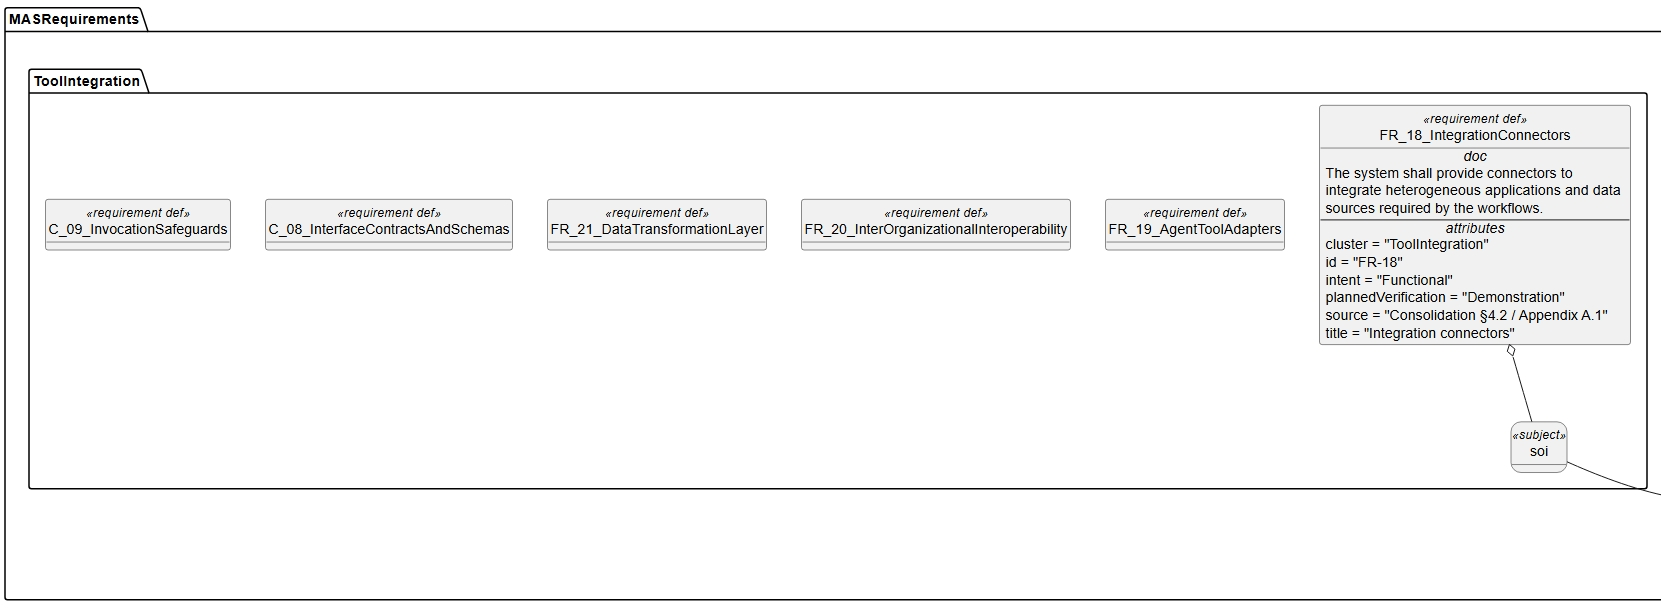
\includegraphics[width=\linewidth]{ressources/MAS/diagrams/MASRequirements/MASRequirements1}
\end{figure}
\begin{figure}[H]
  \centering
  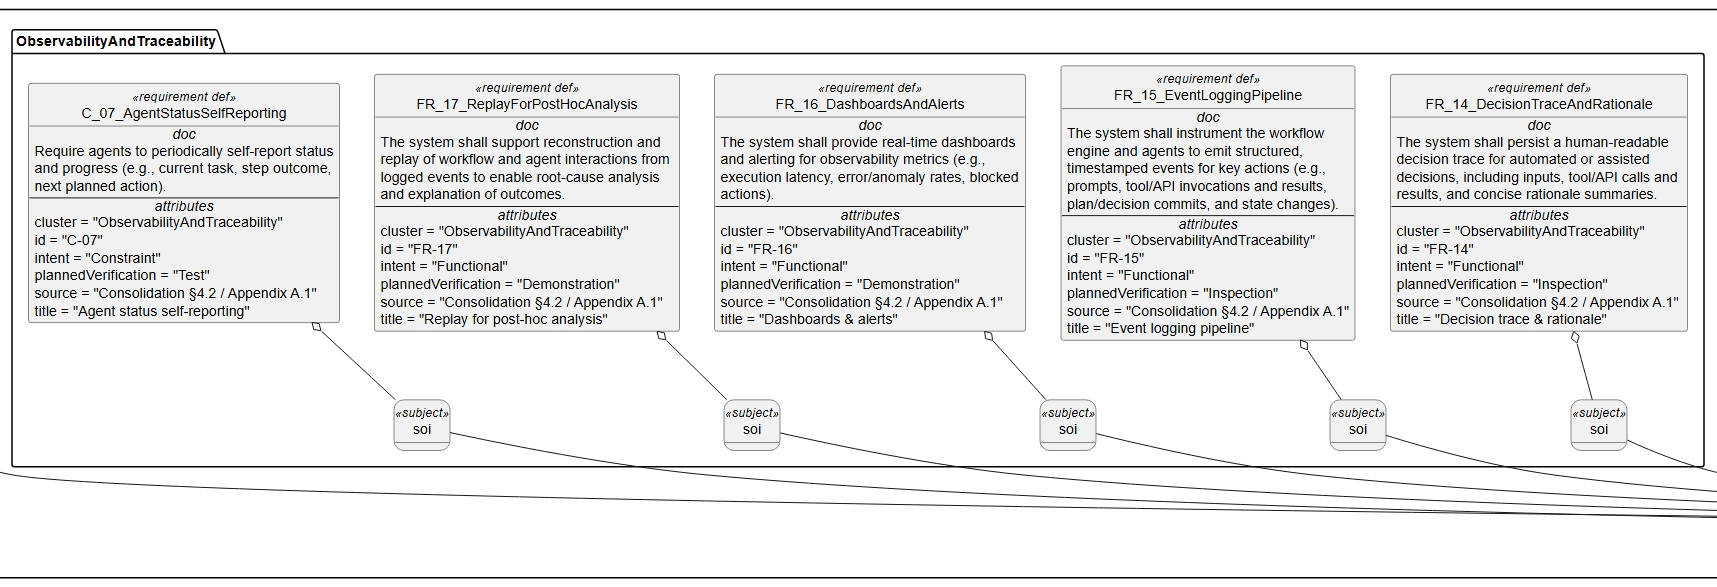
\includegraphics[width=\linewidth]{ressources/MAS/diagrams/MASRequirements/MASRequirements2}
\end{figure}
\begin{figure}[H]
  \centering
  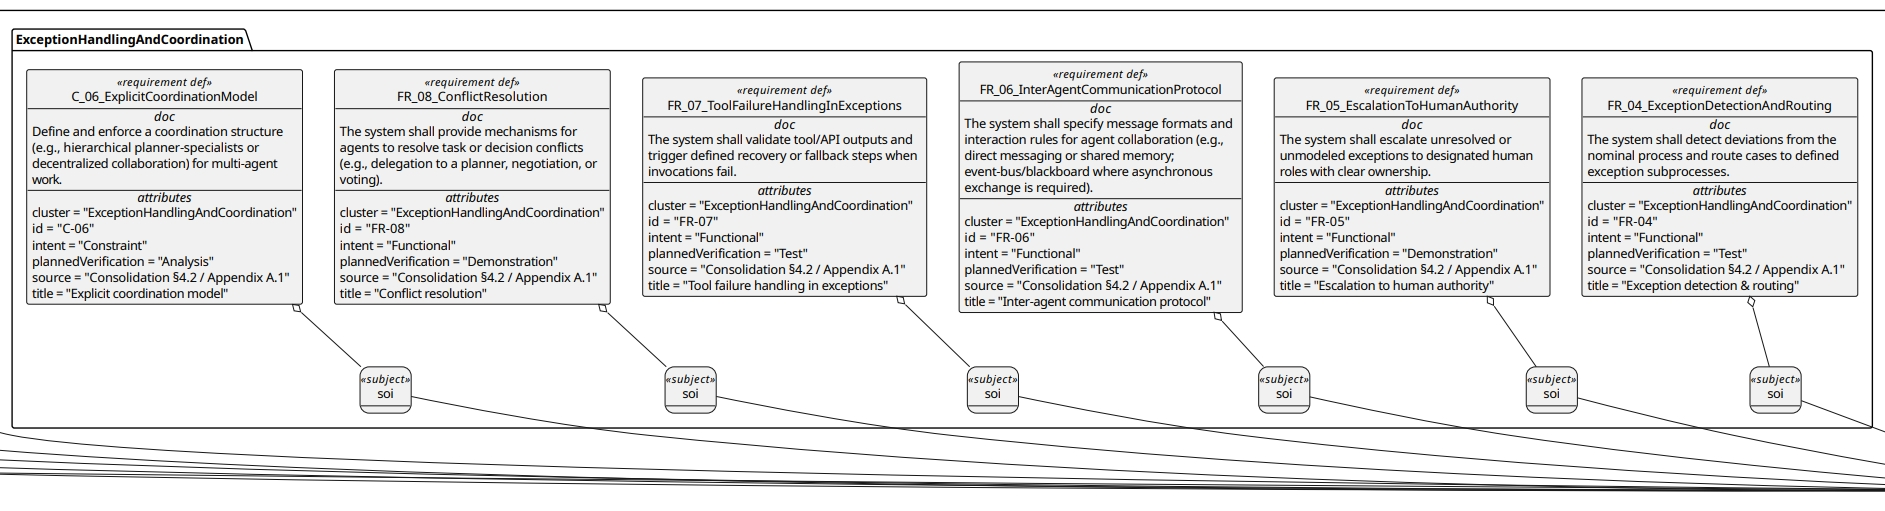
\includegraphics[width=\linewidth]{ressources/MAS/diagrams/MASRequirements/MASRequirements3}
\end{figure}
\begin{figure}[H]
  \centering
  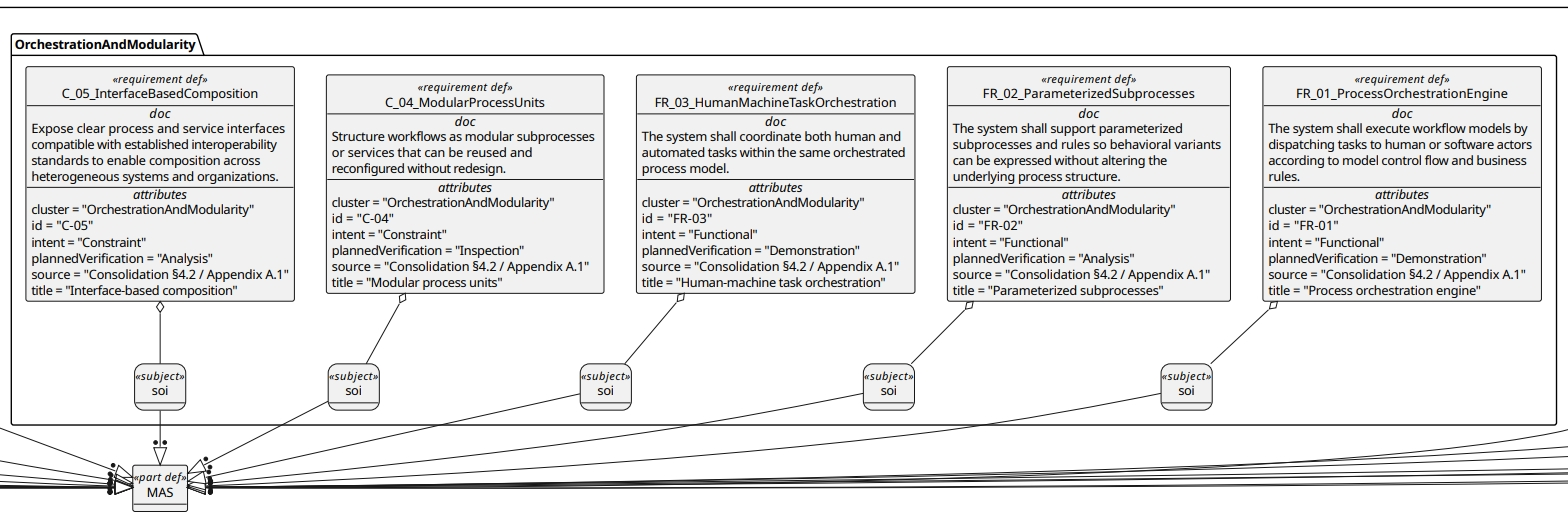
\includegraphics[width=\linewidth]{ressources/MAS/diagrams/MASRequirements/MASRequirements4}
\end{figure}
\begin{figure}[H]
  \centering
  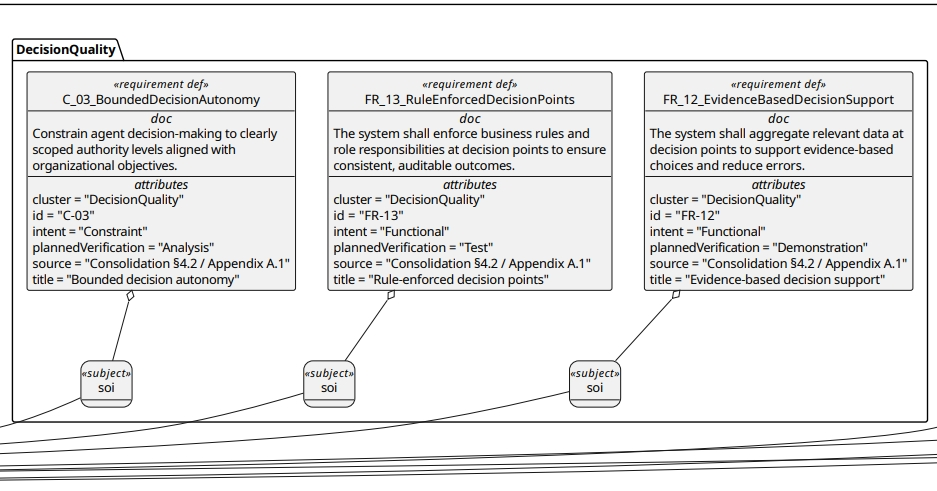
\includegraphics[width=\linewidth]{ressources/MAS/diagrams/MASRequirements/MASRequirements5}
\end{figure}
\begin{figure}[H]
  \centering
  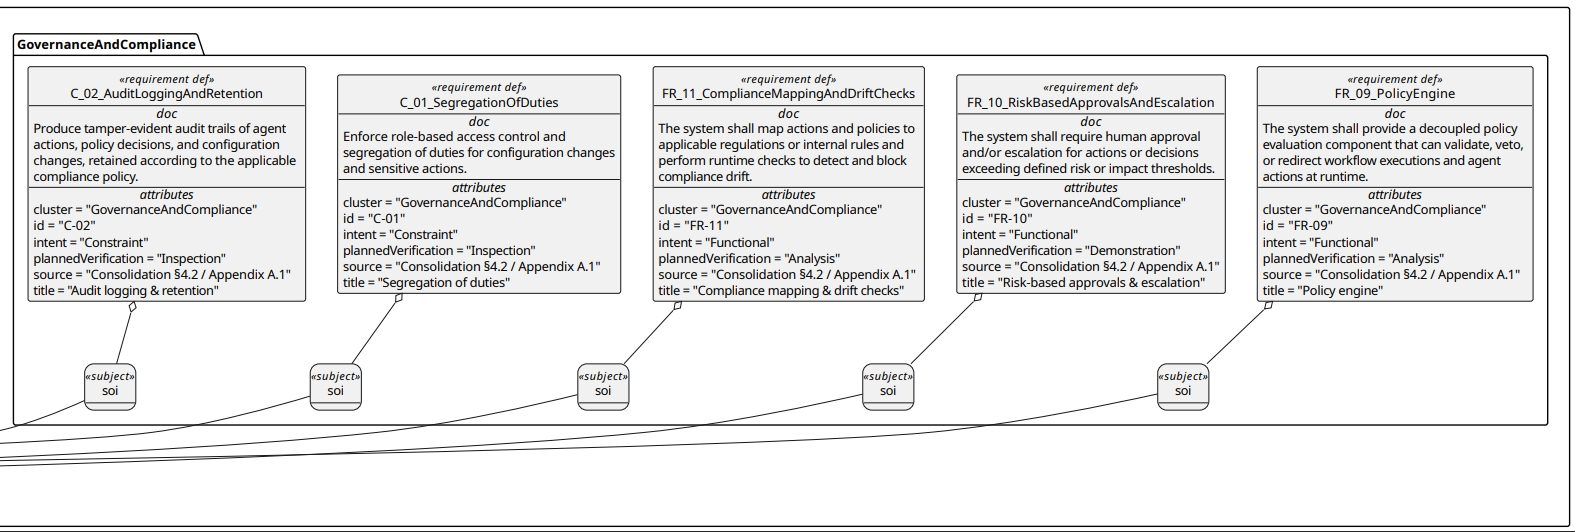
\includegraphics[width=\linewidth]{ressources/MAS/diagrams/MASRequirements/MASRequirements6}
\end{figure}
\clearpage
\lstinputlisting[
  style=sysml,
  label={lst:mas-reqs},
  numbers=left,
  inputencoding=utf8
]{./ressources/MAS/MASRequirements.sysml}

% \subsection*{B.1 Architecture SysML v2 Model}
% \begin{figure}[H]
%   \centering
%   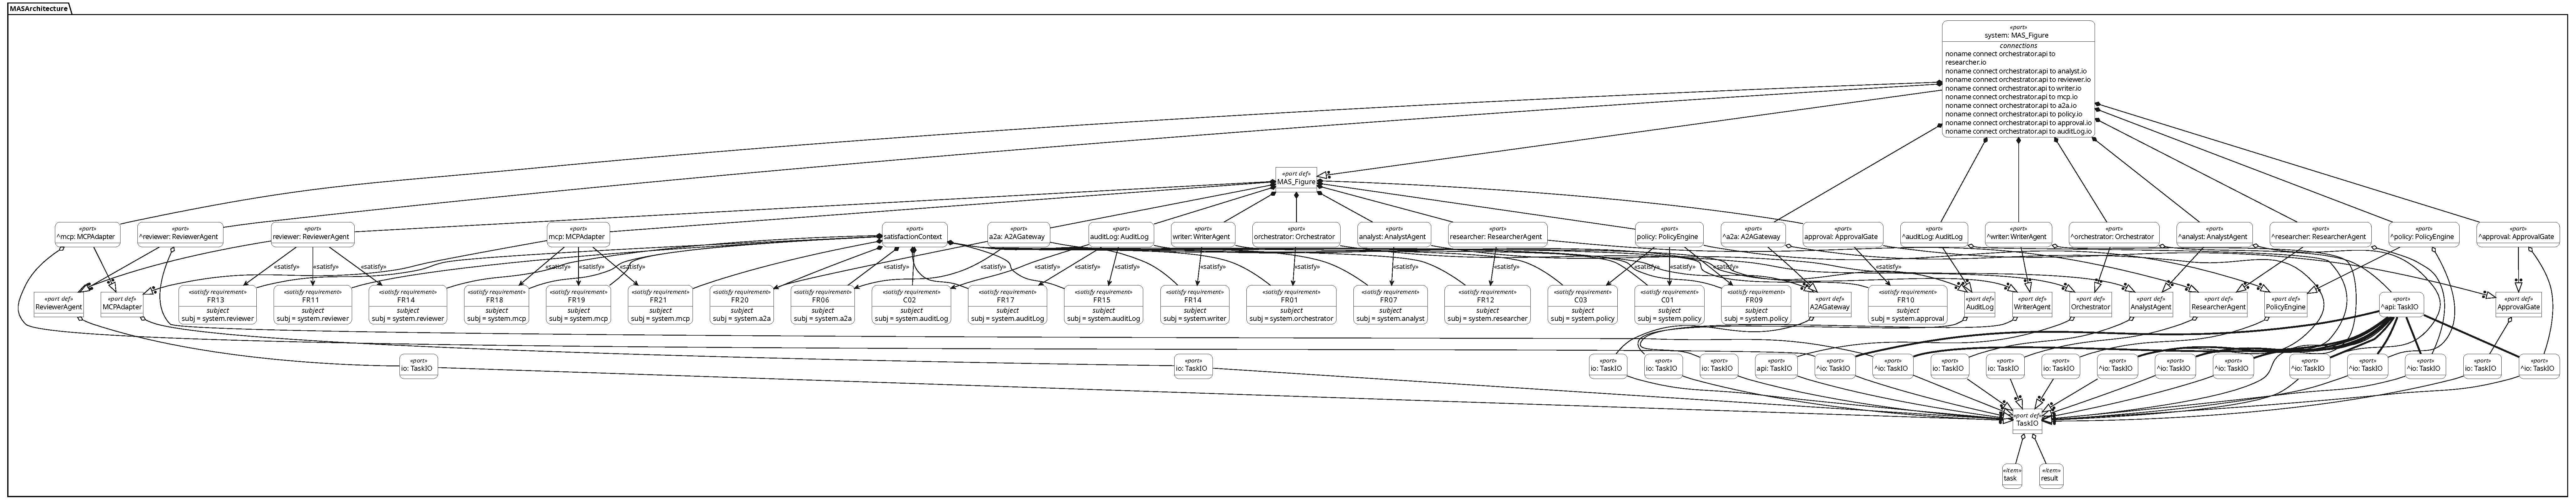
\includegraphics[width=\linewidth]{ressources/MAS/diagrams/MASArchitecture.pdf}\label{fig:arch}
% \end{figure}

% \lstinputlisting[
%   style=sysml,
%   label={lst:mas-arch},
%   inputencoding=utf8
% ]{./ressources/MAS/MASArchitecture.sysml}

% \subsection*{B.2 Architecture Figure}
% \begin{figure}[H]
%   \centering
%   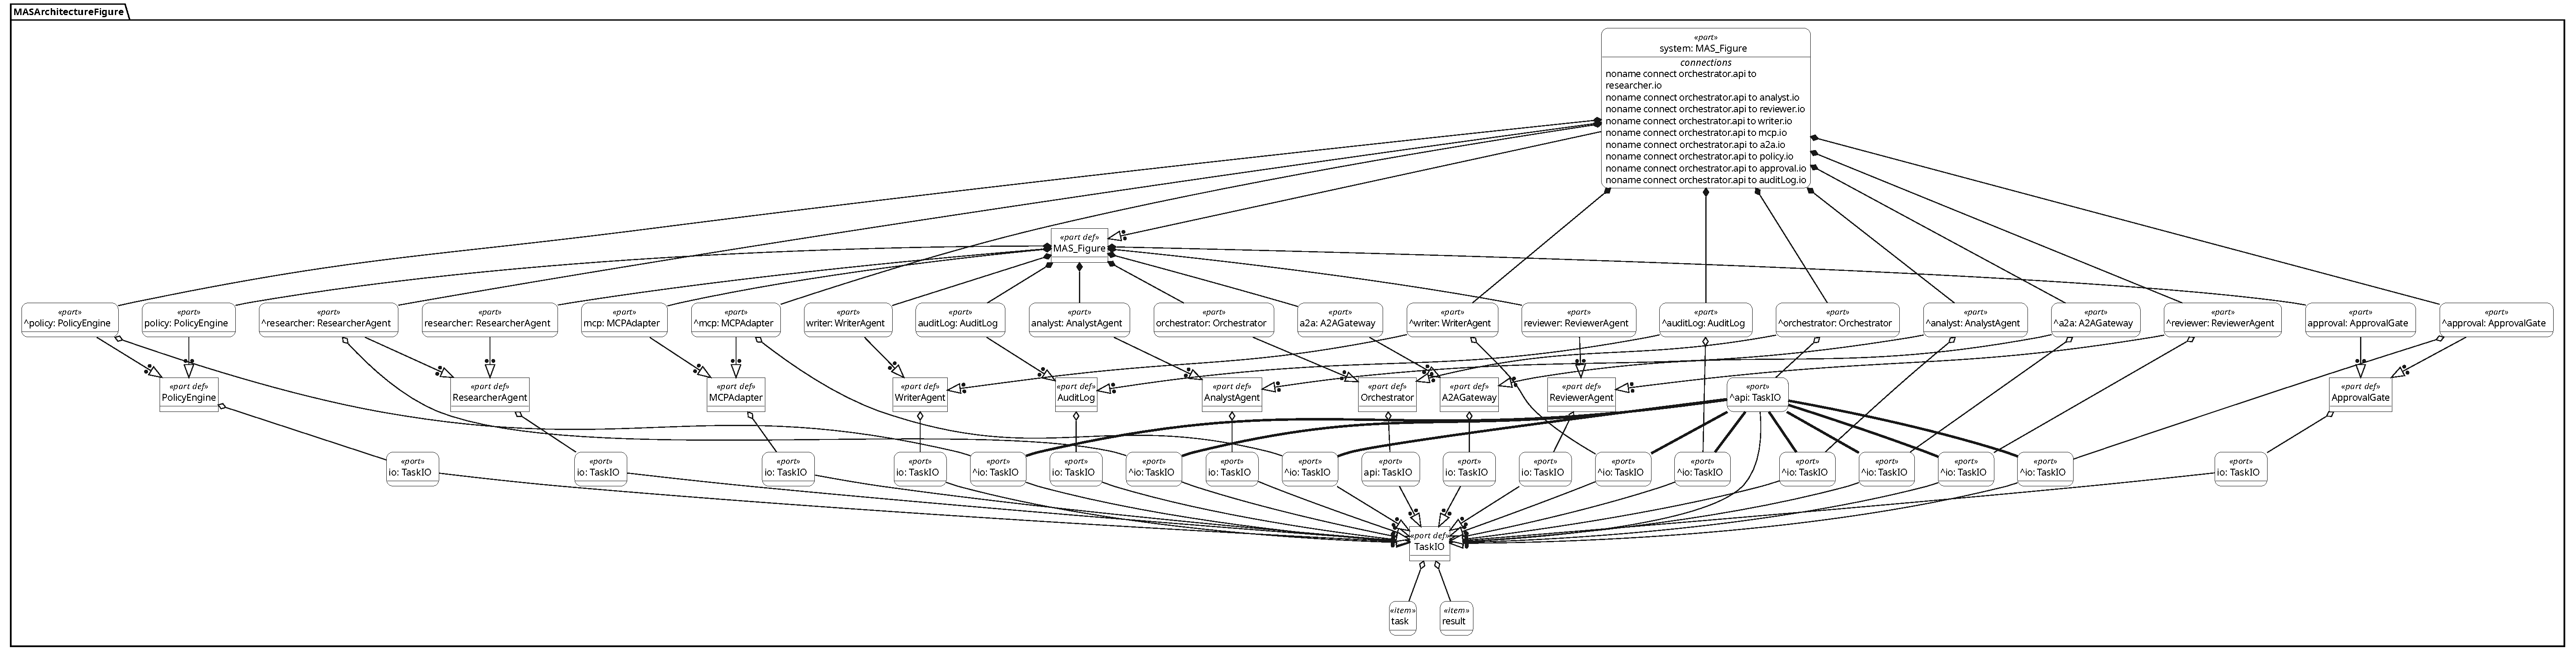
\includegraphics[width=\linewidth]{ressources/MAS/diagrams/MASArchitecture_Figure.pdf}\label{fig:arch-fig}
% \end{figure}

% \subsection*{B.3 Architecture Figure SysML v2 Code}
% \lstinputlisting[
%   style=sysml,
%   caption={Architecture figure (MASArchitecture\_Figure.sysml)},
%   label={lst:mas-arch-figure},
%   inputencoding=utf8
% ]{./ressources/MAS/MASArchitecture_Figure.sysml}

% \subsection*{C.1 Traceability Diagram}
% \begin{figure}[H]
%   \centering
%   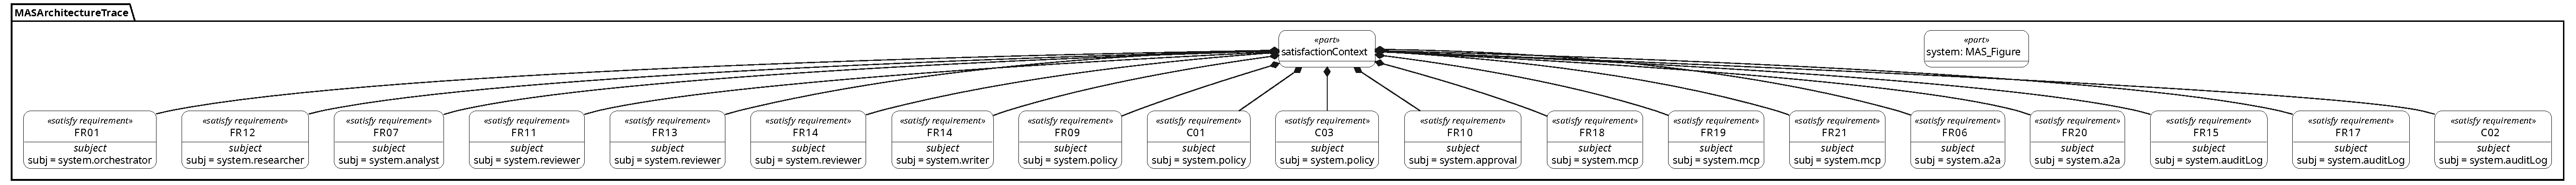
\includegraphics[width=\linewidth]{ressources/MAS/diagrams/MASArchitecture_Trace.pdf}\label{fig:trace}
% \end{figure}

% \subsection*{C.2 Traceability SysML v2 Code}
% \lstinputlisting[
%   style=sysml,
%   caption={Traceability mapping (MASArchitecture\_Trace.sysml)},
%   label={lst:mas-arch-trace},
%   inputencoding=utf8
% ]{./ressources/MAS/MASArchitecture_Trace.sysml}

% \subsection*{C. 3 Traceability}
% \begin{figure}[H]
%   \centering
%   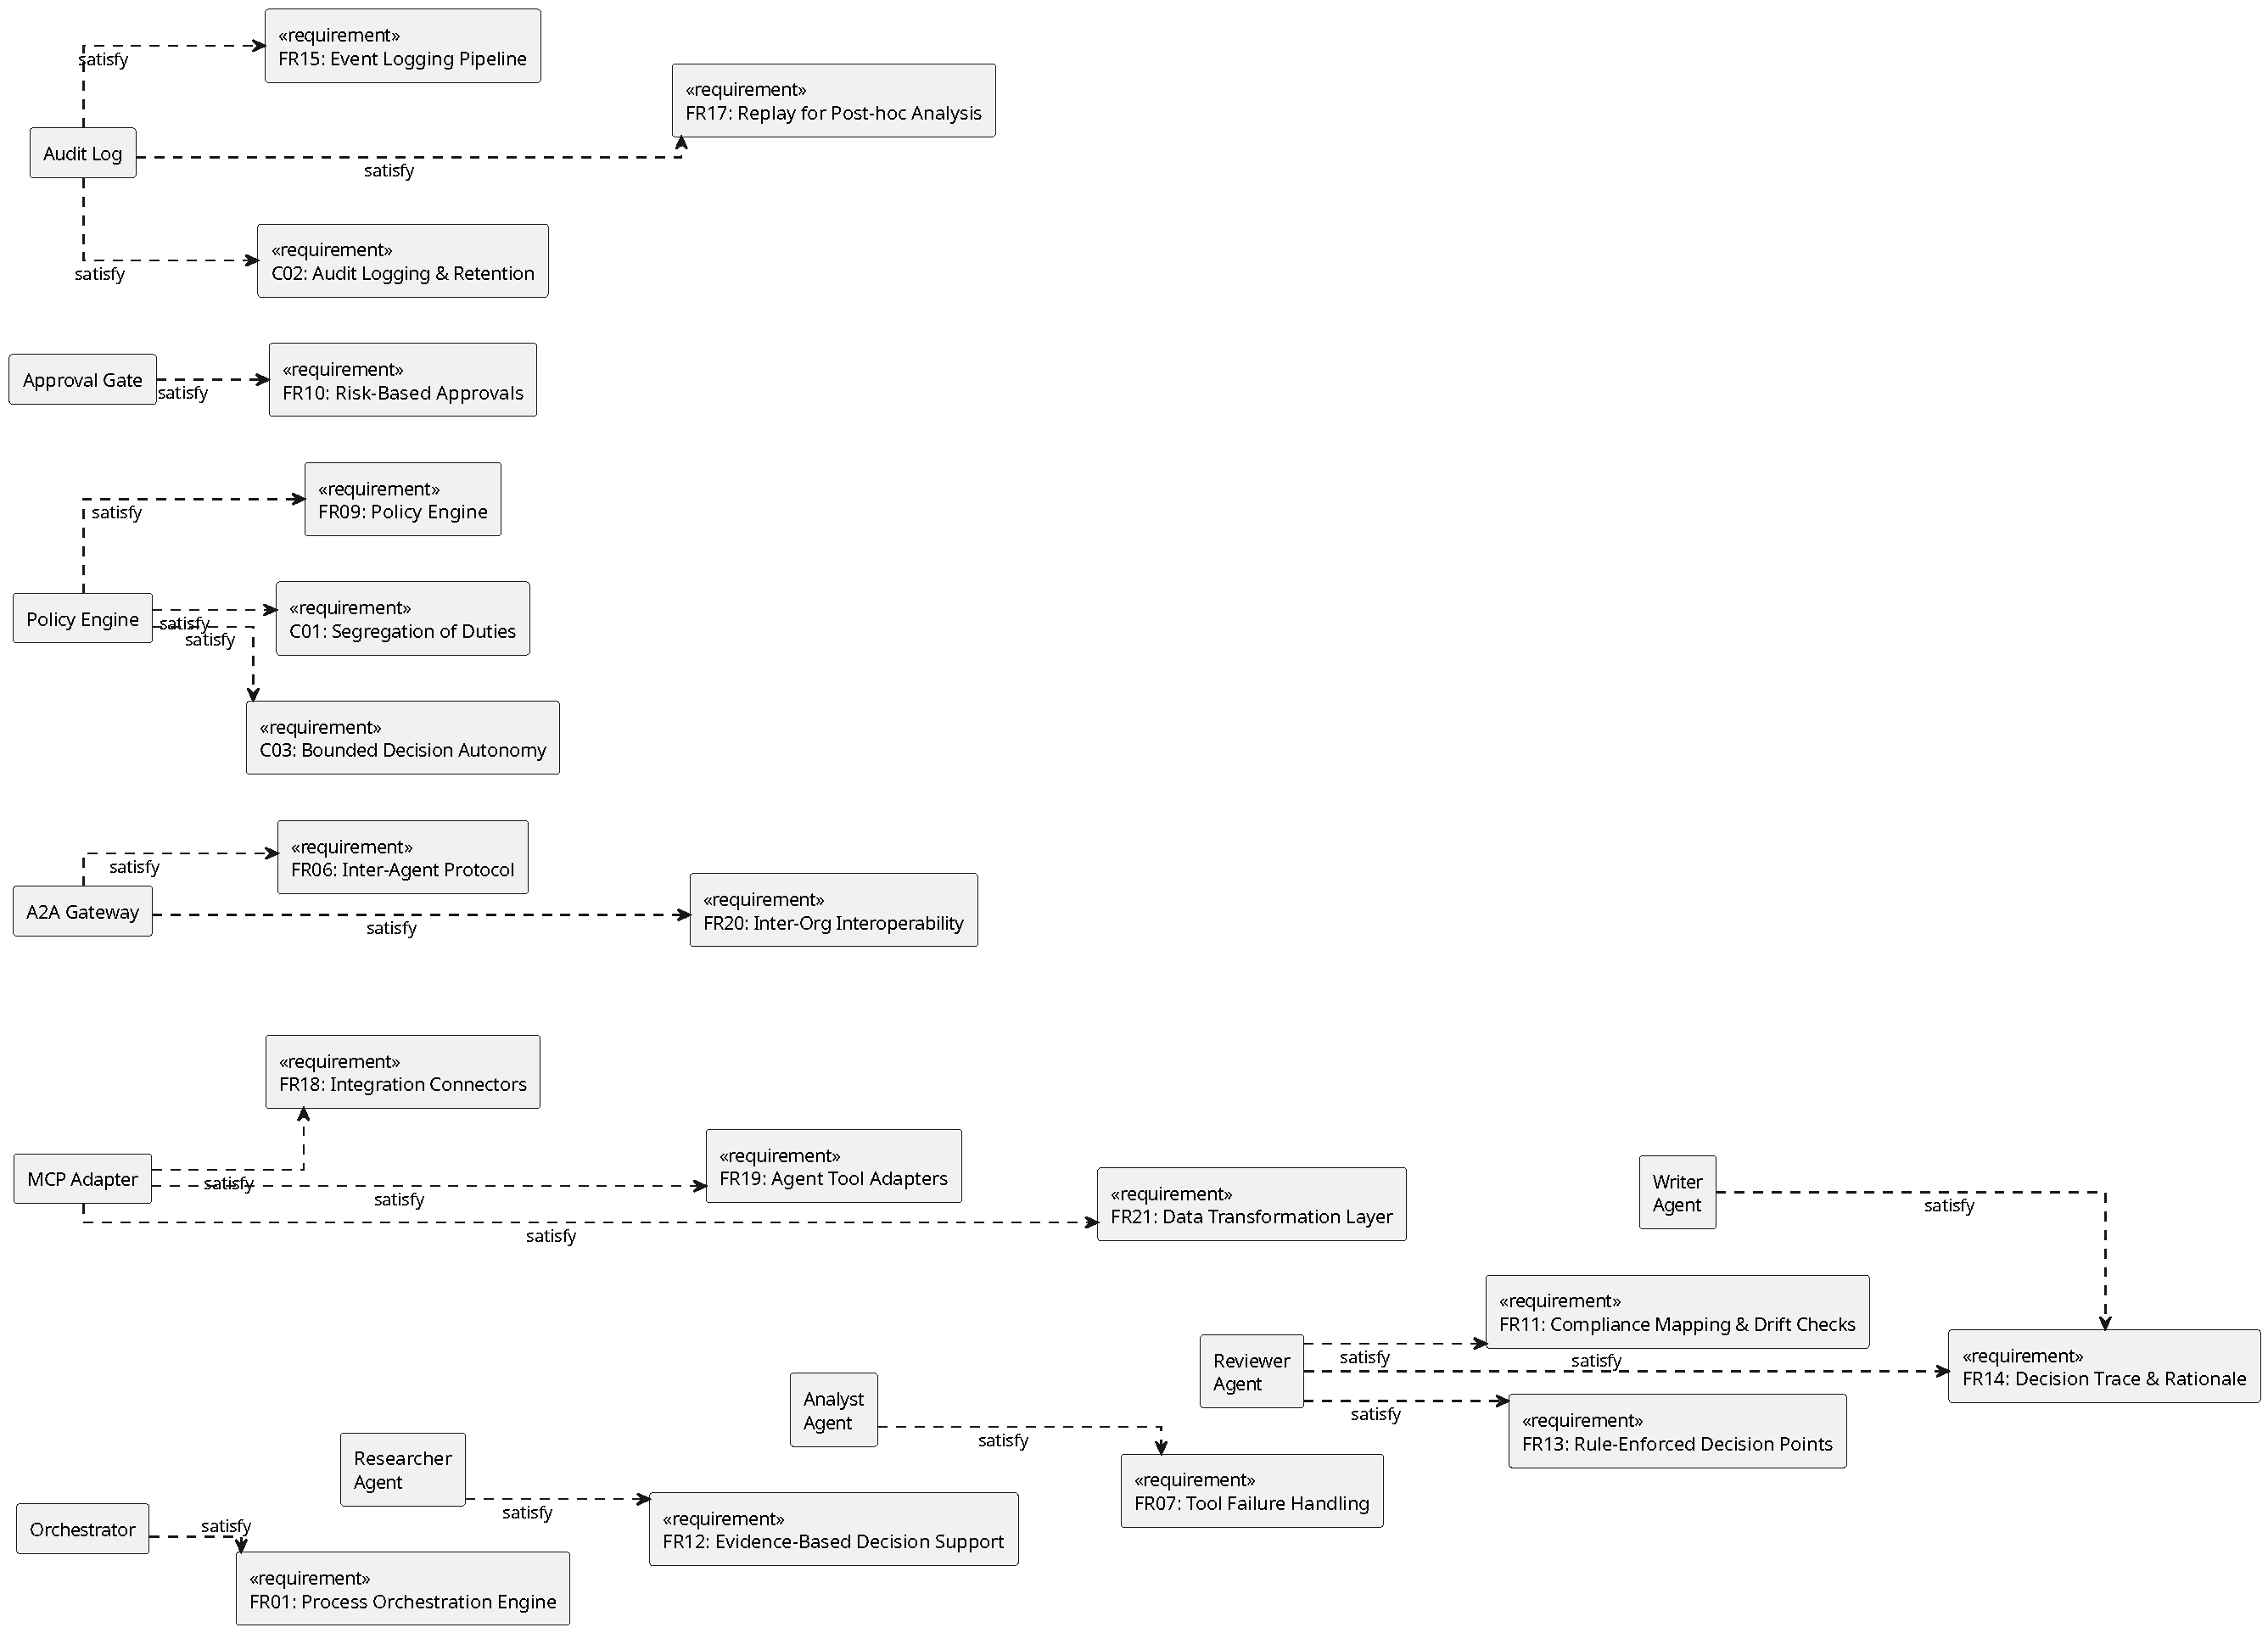
\includegraphics[width=\linewidth]{ressources/MAS/diagrams/fig-traceability.pdf}\label{fig:trace-fig}
% \end{figure}

% --- NDA ---
% \clearpage
% \thispagestyle{empty}
% \begin{center}
% 	\vspace*{1cm}
% 	\Huge\textbf{Non-Disclosure Agreement}\\
% 	\vspace*{2cm}
% 	\normalsize
% 	\begin{quotation}
% 		\parbox{0.8\textwidth}{The present bachelor's thesis contains internal confidential information of the company \myCompany, \myCompanyAddress. The dissemination of the content of the work in whole or in part is strictly prohibited. No copies or transcripts, including digital forms, cane made. Exceptions require the written approval of the company \myCompany.}
% 	\end{quotation}
% 	\vspace*{1cm}
% 	\begin{quotation}
% 		\parbox{0.8\textwidth}{
% 		\begin{tabularx}{0.78\textwidth}{l@{\extracolsep\fill}l}
%             \small \myLocation, \today \\
% 	        \rule{6cm}{0.1mm}&\rule{4cm}{0.1mm}\\
% 			Place, Date&Signature
% 		\end{tabularx}}
% 	\end{quotation}
% \end{center}
% \newpage

% --- AI Declaration ---